\documentclass[1p]{elsarticle_modified}
%\bibliographystyle{elsarticle-num}

%\usepackage[colorlinks]{hyperref}
%\usepackage{abbrmath_seonhwa} %\Abb, \Ascr, \Acal ,\Abf, \Afrak
\usepackage{amsfonts}
\usepackage{amssymb}
\usepackage{amsmath}
\usepackage{amsthm}
\usepackage{scalefnt}
\usepackage{amsbsy}
\usepackage{kotex}
\usepackage{caption}
\usepackage{subfig}
\usepackage{color}
\usepackage{graphicx}
\usepackage{xcolor} %% white, black, red, green, blue, cyan, magenta, yellow
\usepackage{float}
\usepackage{setspace}
\usepackage{hyperref}

\usepackage{tikz}
\usetikzlibrary{arrows}

\usepackage{multirow}
\usepackage{array} % fixed length table
\usepackage{hhline}

%%%%%%%%%%%%%%%%%%%%%
\makeatletter
\renewcommand*\env@matrix[1][\arraystretch]{%
	\edef\arraystretch{#1}%
	\hskip -\arraycolsep
	\let\@ifnextchar\new@ifnextchar
	\array{*\c@MaxMatrixCols c}}
\makeatother %https://tex.stackexchange.com/questions/14071/how-can-i-increase-the-line-spacing-in-a-matrix
%%%%%%%%%%%%%%%

\usepackage[normalem]{ulem}

\newcommand{\msout}[1]{\ifmmode\text{\sout{\ensuremath{#1}}}\else\sout{#1}\fi}
%SOURCE: \msout is \stkout macro in https://tex.stackexchange.com/questions/20609/strikeout-in-math-mode

\newcommand{\cancel}[1]{
	\ifmmode
	{\color{red}\msout{#1}}
	\else
	{\color{red}\sout{#1}}
	\fi
}

\newcommand{\add}[1]{
	{\color{blue}\uwave{#1}}
}

\newcommand{\replace}[2]{
	\ifmmode
	{\color{red}\msout{#1}}{\color{blue}\uwave{#2}}
	\else
	{\color{red}\sout{#1}}{\color{blue}\uwave{#2}}
	\fi
}

\newcommand{\Sol}{\mathcal{S}} %segment
\newcommand{\D}{D} %diagram
\newcommand{\A}{\mathcal{A}} %arc


%%%%%%%%%%%%%%%%%%%%%%%%%%%%%5 test

\def\sl{\operatorname{\textup{SL}}(2,\Cbb)}
\def\psl{\operatorname{\textup{PSL}}(2,\Cbb)}
\def\quan{\mkern 1mu \triangleright \mkern 1mu}

\theoremstyle{definition}
\newtheorem{thm}{Theorem}[section]
\newtheorem{prop}[thm]{Proposition}
\newtheorem{lem}[thm]{Lemma}
\newtheorem{ques}[thm]{Question}
\newtheorem{cor}[thm]{Corollary}
\newtheorem{defn}[thm]{Definition}
\newtheorem{exam}[thm]{Example}
\newtheorem{rmk}[thm]{Remark}
\newtheorem{alg}[thm]{Algorithm}

\newcommand{\I}{\sqrt{-1}}
\begin{document}

%\begin{frontmatter}
%
%\title{Boundary parabolic representations of knots up to 8 crossings}
%
%%% Group authors per affiliation:
%\author{Yunhi Cho} 
%\address{Department of Mathematics, University of Seoul, Seoul, Korea}
%\ead{yhcho@uos.ac.kr}
%
%
%\author{Seonhwa Kim} %\fnref{s_kim}}
%\address{Center for Geometry and Physics, Institute for Basic Science, Pohang, 37673, Korea}
%\ead{ryeona17@ibs.re.kr}
%
%\author{Hyuk Kim}
%\address{Department of Mathematical Sciences, Seoul National University, Seoul 08826, Korea}
%\ead{hyukkim@snu.ac.kr}
%
%\author{Seokbeom Yoon}
%\address{Department of Mathematical Sciences, Seoul National University, Seoul, 08826,  Korea}
%\ead{sbyoon15@snu.ac.kr}
%
%\begin{abstract}
%We find all boundary parabolic representation of knots up to 8 crossings.
%
%\end{abstract}
%\begin{keyword}
%    \MSC[2010] 57M25 
%\end{keyword}
%
%\end{frontmatter}

%\linenumbers
%\tableofcontents
%
\newcommand\colored[1]{\textcolor{white}{\rule[-0.35ex]{0.8em}{1.4ex}}\kern-0.8em\color{red} #1}%
%\newcommand\colored[1]{\textcolor{white}{ #1}\kern-2.17ex	\textcolor{white}{ #1}\kern-1.81ex	\textcolor{white}{ #1}\kern-2.15ex\color{red}#1	}

{\Large $\underline{12n_{0070}~(K12n_{0070})}$}

\setlength{\tabcolsep}{10pt}
\renewcommand{\arraystretch}{1.6}
\vspace{1cm}\begin{tabular}{m{100pt}>{\centering\arraybackslash}m{274pt}}
\multirow{5}{120pt}{
	\centering
	\includegraphics[width=112pt]{../../../GIT/diagram.site/Diagrams/png/2159_12n_0070.png}\\
\ \ \ A knot diagram\footnotemark}&
\allowdisplaybreaks
\textbf{Linearized knot diagam} \\
\cline{2-2}
 &
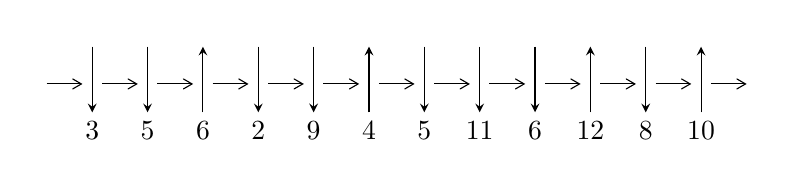
\begin{tikzpicture}[x=20pt, y=17pt]
	% nodes
	\node (C0) at (0, 0) {};
	\node (C1) at (1, 0) {};
	\node (C1U) at (1, +1) {};
	\node (C1D) at (1, -1) {3};

	\node (C2) at (2, 0) {};
	\node (C2U) at (2, +1) {};
	\node (C2D) at (2, -1) {5};

	\node (C3) at (3, 0) {};
	\node (C3U) at (3, +1) {};
	\node (C3D) at (3, -1) {6};

	\node (C4) at (4, 0) {};
	\node (C4U) at (4, +1) {};
	\node (C4D) at (4, -1) {2};

	\node (C5) at (5, 0) {};
	\node (C5U) at (5, +1) {};
	\node (C5D) at (5, -1) {9};

	\node (C6) at (6, 0) {};
	\node (C6U) at (6, +1) {};
	\node (C6D) at (6, -1) {4};

	\node (C7) at (7, 0) {};
	\node (C7U) at (7, +1) {};
	\node (C7D) at (7, -1) {5};

	\node (C8) at (8, 0) {};
	\node (C8U) at (8, +1) {};
	\node (C8D) at (8, -1) {11};

	\node (C9) at (9, 0) {};
	\node (C9U) at (9, +1) {};
	\node (C9D) at (9, -1) {6};

	\node (C10) at (10, 0) {};
	\node (C10U) at (10, +1) {};
	\node (C10D) at (10, -1) {12};

	\node (C11) at (11, 0) {};
	\node (C11U) at (11, +1) {};
	\node (C11D) at (11, -1) {8};

	\node (C12) at (12, 0) {};
	\node (C12U) at (12, +1) {};
	\node (C12D) at (12, -1) {10};
	\node (C13) at (13, 0) {};

	% arrows
	\draw[->,>={angle 60}]
	(C0) edge (C1) (C1) edge (C2) (C2) edge (C3) (C3) edge (C4) (C4) edge (C5) (C5) edge (C6) (C6) edge (C7) (C7) edge (C8) (C8) edge (C9) (C9) edge (C10) (C10) edge (C11) (C11) edge (C12) (C12) edge (C13) ;	\draw[->,>=stealth]
	(C1U) edge (C1D) (C2U) edge (C2D) (C3D) edge (C3U) (C4U) edge (C4D) (C5U) edge (C5D) (C6D) edge (C6U) (C7U) edge (C7D) (C8U) edge (C8D) (C9U) edge (C9D) (C10D) edge (C10U) (C11U) edge (C11D) (C12D) edge (C12U) ;
	\end{tikzpicture} \\
\hhline{~~} \\& 
\textbf{Solving Sequence} \\ \cline{2-2} 
 &
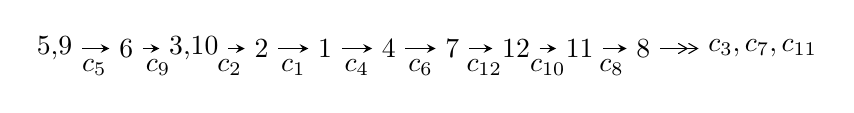
\begin{tikzpicture}[x=23pt, y=7pt]
	% node
	\node (A0) at (-1/8, 0) {5,9};
	\node (A1) at (1, 0) {6};
	\node (A2) at (33/16, 0) {3,10};
	\node (A3) at (25/8, 0) {2};
	\node (A4) at (33/8, 0) {1};
	\node (A5) at (41/8, 0) {4};
	\node (A6) at (49/8, 0) {7};
	\node (A7) at (57/8, 0) {12};
	\node (A8) at (65/8, 0) {11};
	\node (A9) at (73/8, 0) {8};
	\node (C1) at (1/2, -1) {$c_{5}$};
	\node (C2) at (3/2, -1) {$c_{9}$};
	\node (C3) at (21/8, -1) {$c_{2}$};
	\node (C4) at (29/8, -1) {$c_{1}$};
	\node (C5) at (37/8, -1) {$c_{4}$};
	\node (C6) at (45/8, -1) {$c_{6}$};
	\node (C7) at (53/8, -1) {$c_{12}$};
	\node (C8) at (61/8, -1) {$c_{10}$};
	\node (C9) at (69/8, -1) {$c_{8}$};
	\node (A10) at (11, 0) {$c_{3},c_{7},c_{11}$};

	% edge
	\draw[->,>=stealth]	
	(A0) edge (A1) (A1) edge (A2) (A2) edge (A3) (A3) edge (A4) (A4) edge (A5) (A5) edge (A6) (A6) edge (A7) (A7) edge (A8) (A8) edge (A9) ;
	\draw[->>,>={angle 60}]	
	(A9) edge (A10);
\end{tikzpicture} \\ 

\end{tabular} \\

\footnotetext{
The image of knot diagram is generated by the software ``\textbf{Draw programme}" developed by Andrew Bartholomew(\url{http://www.layer8.co.uk/maths/draw/index.htm\#Running-draw}), where we modified some parts for our purpose(\url{https://github.com/CATsTAILs/LinksPainter}).
}\phantom \\ \newline 
\centering \textbf{Ideals for irreducible components\footnotemark of $X_{\text{par}}$} 
 
\begin{align*}
I^u_{1}&=\langle 
-2.79874\times10^{43} u^{47}+4.02119\times10^{43} u^{46}+\cdots+8.11774\times10^{44} b+8.69331\times10^{44},\\
\phantom{I^u_{1}}&\phantom{= \langle  }8.37339\times10^{44} u^{47}-7.89584\times10^{44} u^{46}+\cdots+8.11774\times10^{44} a+8.23673\times10^{44},\;u^{48}-2 u^{47}+\cdots+u-1\rangle \\
I^u_{2}&=\langle 
b+1,\;- u^8+3 u^6+u^5-4 u^4-2 u^3+u^2+a+2 u+1,\;u^9+u^8-2 u^7-3 u^6+u^5+3 u^4+2 u^3- u-1\rangle \\
\\
\end{align*}
\raggedright * 2 irreducible components of $\dim_{\mathbb{C}}=0$, with total 57 representations.\\
\footnotetext{All coefficients of polynomials are rational numbers. But the coefficients are sometimes approximated in decimal forms when there is not enough margin.}
\newpage
\renewcommand{\arraystretch}{1}
\centering \section*{I. $I^u_{1}= \langle -2.80\times10^{43} u^{47}+4.02\times10^{43} u^{46}+\cdots+8.12\times10^{44} b+8.69\times10^{44},\;8.37\times10^{44} u^{47}-7.90\times10^{44} u^{46}+\cdots+8.12\times10^{44} a+8.24\times10^{44},\;u^{48}-2 u^{47}+\cdots+u-1 \rangle$}
\flushleft \textbf{(i) Arc colorings}\\
\begin{tabular}{m{7pt} m{180pt} m{7pt} m{180pt} }
\flushright $a_{5}=$&$\begin{pmatrix}1\\0\end{pmatrix}$ \\
\flushright $a_{9}=$&$\begin{pmatrix}0\\u\end{pmatrix}$ \\
\flushright $a_{6}=$&$\begin{pmatrix}1\\u^2\end{pmatrix}$ \\
\flushright $a_{3}=$&$\begin{pmatrix}-1.03149 u^{47}+0.972665 u^{46}+\cdots+7.94786 u-1.01466\\0.0344769 u^{47}-0.0495358 u^{46}+\cdots+0.0738871 u-1.07090\end{pmatrix}$ \\
\flushright $a_{10}=$&$\begin{pmatrix}- u\\- u^3+u\end{pmatrix}$ \\
\flushright $a_{2}=$&$\begin{pmatrix}-0.997016 u^{47}+0.923129 u^{46}+\cdots+8.02175 u-2.08556\\0.0344769 u^{47}-0.0495358 u^{46}+\cdots+0.0738871 u-1.07090\end{pmatrix}$ \\
\flushright $a_{1}=$&$\begin{pmatrix}0.0331947 u^{47}-0.0856097 u^{46}+\cdots+0.0573894 u-1.12853\\0.0134332 u^{47}-0.0242057 u^{46}+\cdots+0.0350763 u-0.0500498\end{pmatrix}$ \\
\flushright $a_{4}=$&$\begin{pmatrix}-1.02750 u^{47}+0.980811 u^{46}+\cdots+7.96292 u-0.995240\\0.0271246 u^{47}-0.0401768 u^{46}+\cdots+0.0617487 u-1.05477\end{pmatrix}$ \\
\flushright $a_{7}=$&$\begin{pmatrix}0.0331947 u^{47}-0.0856097 u^{46}+\cdots+0.0573894 u-1.12853\\0.0231038 u^{47}-0.00484707 u^{46}+\cdots+0.0173387 u+0.0308295\end{pmatrix}$ \\
\flushright $a_{12}=$&$\begin{pmatrix}0.00227898 u^{47}-0.0424799 u^{46}+\cdots-0.0132823 u-1.06795\\0.0555135 u^{47}-0.0910188 u^{46}+\cdots+0.0935339 u-0.129332\end{pmatrix}$ \\
\flushright $a_{11}=$&$\begin{pmatrix}-0.00405982 u^{47}+0.347568 u^{46}+\cdots-0.370675 u+0.256769\\0.0520834 u^{47}-0.385513 u^{46}+\cdots+0.537247 u+0.0988580\end{pmatrix}$ \\
\flushright $a_{8}=$&$\begin{pmatrix}0.0100910 u^{47}-0.0807626 u^{46}+\cdots+0.0400507 u-1.15936\\0.0231038 u^{47}-0.00484707 u^{46}+\cdots+0.0173387 u+0.0308295\end{pmatrix}$\\&\end{tabular}
\flushleft \textbf{(ii) Obstruction class $= -1$}\\~\\
\flushleft \textbf{(iii) Cusp Shapes $= -5.65697 u^{47}+10.4260 u^{46}+\cdots+9.56539 u-4.59345$}\\~\\
\newpage\renewcommand{\arraystretch}{1}
\flushleft \textbf{(iv) u-Polynomials at the component}\newline \\
\begin{tabular}{m{50pt}|m{274pt}}
Crossings & \hspace{64pt}u-Polynomials at each crossing \\
\hline $$\begin{aligned}c_{1}\end{aligned}$$&$\begin{aligned}
&u^{48}+10 u^{47}+\cdots+29 u+1
\end{aligned}$\\
\hline $$\begin{aligned}c_{2},c_{4}\end{aligned}$$&$\begin{aligned}
&u^{48}-10 u^{47}+\cdots+9 u-1
\end{aligned}$\\
\hline $$\begin{aligned}c_{3},c_{6}\end{aligned}$$&$\begin{aligned}
&u^{48}+5 u^{47}+\cdots+2560 u+512
\end{aligned}$\\
\hline $$\begin{aligned}c_{5},c_{9}\end{aligned}$$&$\begin{aligned}
&u^{48}+2 u^{47}+\cdots- u-1
\end{aligned}$\\
\hline $$\begin{aligned}c_{7}\end{aligned}$$&$\begin{aligned}
&u^{48}-10 u^{47}+\cdots-284463 u-118529
\end{aligned}$\\
\hline $$\begin{aligned}c_{8},c_{11}\end{aligned}$$&$\begin{aligned}
&u^{48}-2 u^{47}+\cdots+5 u+1
\end{aligned}$\\
\hline $$\begin{aligned}c_{10},c_{12}\end{aligned}$$&$\begin{aligned}
&u^{48}-18 u^{47}+\cdots+5 u+1
\end{aligned}$\\
\hline
\end{tabular}\\~\\
\newpage\renewcommand{\arraystretch}{1}
\flushleft \textbf{(v) Riley Polynomials at the component}\newline \\
\begin{tabular}{m{50pt}|m{274pt}}
Crossings & \hspace{64pt}Riley Polynomials at each crossing \\
\hline $$\begin{aligned}c_{1}\end{aligned}$$&$\begin{aligned}
&y^{48}+66 y^{47}+\cdots-29 y+1
\end{aligned}$\\
\hline $$\begin{aligned}c_{2},c_{4}\end{aligned}$$&$\begin{aligned}
&y^{48}-10 y^{47}+\cdots-29 y+1
\end{aligned}$\\
\hline $$\begin{aligned}c_{3},c_{6}\end{aligned}$$&$\begin{aligned}
&y^{48}-57 y^{47}+\cdots-6553600 y+262144
\end{aligned}$\\
\hline $$\begin{aligned}c_{5},c_{9}\end{aligned}$$&$\begin{aligned}
&y^{48}-10 y^{47}+\cdots-5 y+1
\end{aligned}$\\
\hline $$\begin{aligned}c_{7}\end{aligned}$$&$\begin{aligned}
&y^{48}+46 y^{47}+\cdots+130798249663 y+14049123841
\end{aligned}$\\
\hline $$\begin{aligned}c_{8},c_{11}\end{aligned}$$&$\begin{aligned}
&y^{48}+18 y^{47}+\cdots-5 y+1
\end{aligned}$\\
\hline $$\begin{aligned}c_{10},c_{12}\end{aligned}$$&$\begin{aligned}
&y^{48}+26 y^{47}+\cdots-305 y+1
\end{aligned}$\\
\hline
\end{tabular}\\~\\
\newpage\flushleft \textbf{(vi) Complex Volumes and Cusp Shapes}
$$\begin{array}{c|c|c}  
\text{Solutions to }I^u_{1}& \I (\text{vol} + \sqrt{-1}CS) & \text{Cusp shape}\\
 \hline 
\begin{aligned}
u &= -0.896760 + 0.394007 I \\
a &= \phantom{-}1.195670 + 0.370079 I \\
b &= \phantom{-}0.334698 - 0.383487 I\end{aligned}
 & \phantom{-}1.62098 + 2.77574 I & \phantom{-}0.84836 - 5.23754 I \\ \hline\begin{aligned}
u &= -0.896760 - 0.394007 I \\
a &= \phantom{-}1.195670 - 0.370079 I \\
b &= \phantom{-}0.334698 + 0.383487 I\end{aligned}
 & \phantom{-}1.62098 - 2.77574 I & \phantom{-}0.84836 + 5.23754 I \\ \hline\begin{aligned}
u &= \phantom{-}0.974989\phantom{ +0.000000I} \\
a &= \phantom{-}1.02044\phantom{ +0.000000I} \\
b &= \phantom{-}0.393396\phantom{ +0.000000I}\end{aligned}
 & -1.61952\phantom{ +0.000000I} & -5.35010\phantom{ +0.000000I} \\ \hline\begin{aligned}
u &= -0.120610 + 0.916069 I \\
a &= \phantom{-}0.235604 - 0.115451 I \\
b &= \phantom{-}0.343969 + 0.103094 I\end{aligned}
 & -0.93576 - 2.61420 I & -0.93985 + 3.31089 I \\ \hline\begin{aligned}
u &= -0.120610 - 0.916069 I \\
a &= \phantom{-}0.235604 + 0.115451 I \\
b &= \phantom{-}0.343969 - 0.103094 I\end{aligned}
 & -0.93576 + 2.61420 I & -0.93985 - 3.31089 I \\ \hline\begin{aligned}
u &= -0.738807 + 0.549894 I \\
a &= \phantom{-}0.165480 - 1.227210 I \\
b &= -0.486703 + 1.024080 I\end{aligned}
 & -0.48319 + 6.71552 I & -4.51681 - 9.54041 I \\ \hline\begin{aligned}
u &= -0.738807 - 0.549894 I \\
a &= \phantom{-}0.165480 + 1.227210 I \\
b &= -0.486703 - 1.024080 I\end{aligned}
 & -0.48319 - 6.71552 I & -4.51681 + 9.54041 I \\ \hline\begin{aligned}
u &= -0.599663 + 0.680544 I \\
a &= \phantom{-}0.187949 - 0.890060 I \\
b &= -0.049207 + 0.720509 I\end{aligned}
 & \phantom{-}2.76925 + 1.42198 I & \phantom{-}2.53709 - 3.03057 I \\ \hline\begin{aligned}
u &= -0.599663 - 0.680544 I \\
a &= \phantom{-}0.187949 + 0.890060 I \\
b &= -0.049207 - 0.720509 I\end{aligned}
 & \phantom{-}2.76925 - 1.42198 I & \phantom{-}2.53709 + 3.03057 I \\ \hline\begin{aligned}
u &= \phantom{-}0.697412 + 0.490405 I \\
a &= \phantom{-}0.242589 + 1.252710 I \\
b &= -0.620253 - 0.841171 I\end{aligned}
 & -1.49634 - 1.82392 I & -7.12758 + 4.49809 I\\
 \hline 
 \end{array}$$\newpage$$\begin{array}{c|c|c}  
\text{Solutions to }I^u_{1}& \I (\text{vol} + \sqrt{-1}CS) & \text{Cusp shape}\\
 \hline 
\begin{aligned}
u &= \phantom{-}0.697412 - 0.490405 I \\
a &= \phantom{-}0.242589 - 1.252710 I \\
b &= -0.620253 + 0.841171 I\end{aligned}
 & -1.49634 + 1.82392 I & -7.12758 - 4.49809 I \\ \hline\begin{aligned}
u &= \phantom{-}0.741862 + 0.199966 I \\
a &= -0.024215 + 0.937984 I \\
b &= -1.35488 - 0.46391 I\end{aligned}
 & -3.92122 - 4.12814 I & -11.08539 + 6.80823 I \\ \hline\begin{aligned}
u &= \phantom{-}0.741862 - 0.199966 I \\
a &= -0.024215 - 0.937984 I \\
b &= -1.35488 + 0.46391 I\end{aligned}
 & -3.92122 + 4.12814 I & -11.08539 - 6.80823 I \\ \hline\begin{aligned}
u &= -0.732347 + 0.133432 I \\
a &= -0.169686 - 0.690549 I \\
b &= -1.41588 + 0.30582 I\end{aligned}
 & -4.22436 - 0.79348 I & -12.24074 + 0.40151 I \\ \hline\begin{aligned}
u &= -0.732347 - 0.133432 I \\
a &= -0.169686 + 0.690549 I \\
b &= -1.41588 - 0.30582 I\end{aligned}
 & -4.22436 + 0.79348 I & -12.24074 - 0.40151 I \\ \hline\begin{aligned}
u &= -0.837259 + 0.941864 I \\
a &= -0.544783 - 0.719252 I \\
b &= \phantom{-}0.782990 + 1.125810 I\end{aligned}
 & \phantom{-}5.63113 + 1.53351 I & \phantom{-0.000000 } 0 \\ \hline\begin{aligned}
u &= -0.837259 - 0.941864 I \\
a &= -0.544783 + 0.719252 I \\
b &= \phantom{-}0.782990 - 1.125810 I\end{aligned}
 & \phantom{-}5.63113 - 1.53351 I & \phantom{-0.000000 } 0 \\ \hline\begin{aligned}
u &= \phantom{-}0.861555 + 0.923996 I \\
a &= -0.593554 + 0.787088 I \\
b &= \phantom{-}0.79140 - 1.22798 I\end{aligned}
 & \phantom{-}7.43222 - 6.89004 I & \phantom{-0.000000 } 0 \\ \hline\begin{aligned}
u &= \phantom{-}0.861555 - 0.923996 I \\
a &= -0.593554 - 0.787088 I \\
b &= \phantom{-}0.79140 + 1.22798 I\end{aligned}
 & \phantom{-}7.43222 + 6.89004 I & \phantom{-0.000000 } 0 \\ \hline\begin{aligned}
u &= -0.517390 + 0.487120 I \\
a &= \phantom{-}1.92274 - 0.32819 I \\
b &= -0.312068 - 0.327759 I\end{aligned}
 & -0.09198 - 2.92294 I & -2.75678 + 1.45029 I\\
 \hline 
 \end{array}$$\newpage$$\begin{array}{c|c|c}  
\text{Solutions to }I^u_{1}& \I (\text{vol} + \sqrt{-1}CS) & \text{Cusp shape}\\
 \hline 
\begin{aligned}
u &= -0.517390 - 0.487120 I \\
a &= \phantom{-}1.92274 + 0.32819 I \\
b &= -0.312068 + 0.327759 I\end{aligned}
 & -0.09198 + 2.92294 I & -2.75678 - 1.45029 I \\ \hline\begin{aligned}
u &= \phantom{-}0.871406 + 0.978758 I \\
a &= -0.658628 + 0.639461 I \\
b &= \phantom{-}0.95026 - 1.11406 I\end{aligned}
 & \phantom{-}11.29790 + 0.41096 I & \phantom{-0.000000 } 0 \\ \hline\begin{aligned}
u &= \phantom{-}0.871406 - 0.978758 I \\
a &= -0.658628 - 0.639461 I \\
b &= \phantom{-}0.95026 + 1.11406 I\end{aligned}
 & \phantom{-}11.29790 - 0.41096 I & \phantom{-0.000000 } 0 \\ \hline\begin{aligned}
u &= \phantom{-}1.002820 + 0.849357 I \\
a &= \phantom{-}0.72578 - 1.44875 I \\
b &= \phantom{-}0.939578 + 1.008210 I\end{aligned}
 & \phantom{-}6.96696 + 0.32370 I & \phantom{-0.000000 } 0 \\ \hline\begin{aligned}
u &= \phantom{-}1.002820 - 0.849357 I \\
a &= \phantom{-}0.72578 + 1.44875 I \\
b &= \phantom{-}0.939578 - 1.008210 I\end{aligned}
 & \phantom{-}6.96696 - 0.32370 I & \phantom{-0.000000 } 0 \\ \hline\begin{aligned}
u &= \phantom{-}1.271800 + 0.367688 I \\
a &= \phantom{-}0.720656 - 0.331546 I \\
b &= \phantom{-}0.681047 + 0.240011 I\end{aligned}
 & -5.31134 - 1.83633 I & \phantom{-0.000000 } 0 \\ \hline\begin{aligned}
u &= \phantom{-}1.271800 - 0.367688 I \\
a &= \phantom{-}0.720656 + 0.331546 I \\
b &= \phantom{-}0.681047 - 0.240011 I\end{aligned}
 & -5.31134 + 1.83633 I & \phantom{-0.000000 } 0 \\ \hline\begin{aligned}
u &= -0.844944 + 1.021610 I \\
a &= -0.595460 - 0.519471 I \\
b &= \phantom{-}0.959842 + 0.954036 I\end{aligned}
 & \phantom{-}5.10392 - 1.89300 I & \phantom{-0.000000 } 0 \\ \hline\begin{aligned}
u &= -0.844944 - 1.021610 I \\
a &= -0.595460 + 0.519471 I \\
b &= \phantom{-}0.959842 - 0.954036 I\end{aligned}
 & \phantom{-}5.10392 + 1.89300 I & \phantom{-0.000000 } 0 \\ \hline\begin{aligned}
u &= -1.030920 + 0.851423 I \\
a &= \phantom{-}0.63113 + 1.38478 I \\
b &= \phantom{-}0.990071 - 0.940352 I\end{aligned}
 & \phantom{-}5.00640 + 5.09433 I & \phantom{-0.000000 } 0\\
 \hline 
 \end{array}$$\newpage$$\begin{array}{c|c|c}  
\text{Solutions to }I^u_{1}& \I (\text{vol} + \sqrt{-1}CS) & \text{Cusp shape}\\
 \hline 
\begin{aligned}
u &= -1.030920 - 0.851423 I \\
a &= \phantom{-}0.63113 - 1.38478 I \\
b &= \phantom{-}0.990071 + 0.940352 I\end{aligned}
 & \phantom{-}5.00640 - 5.09433 I & \phantom{-0.000000 } 0 \\ \hline\begin{aligned}
u &= -1.266230 + 0.463136 I \\
a &= \phantom{-}0.690484 + 0.432110 I \\
b &= \phantom{-}0.720279 - 0.304393 I\end{aligned}
 & -4.61107 + 7.74308 I & \phantom{-0.000000 } 0 \\ \hline\begin{aligned}
u &= -1.266230 - 0.463136 I \\
a &= \phantom{-}0.690484 - 0.432110 I \\
b &= \phantom{-}0.720279 + 0.304393 I\end{aligned}
 & -4.61107 - 7.74308 I & \phantom{-0.000000 } 0 \\ \hline\begin{aligned}
u &= \phantom{-}0.867259 + 1.032790 I \\
a &= -0.651865 + 0.488809 I \\
b &= \phantom{-}1.034680 - 0.958036 I\end{aligned}
 & \phantom{-}6.65683 + 7.53345 I & \phantom{-0.000000 } 0 \\ \hline\begin{aligned}
u &= \phantom{-}0.867259 - 1.032790 I \\
a &= -0.651865 - 0.488809 I \\
b &= \phantom{-}1.034680 + 0.958036 I\end{aligned}
 & \phantom{-}6.65683 - 7.53345 I & \phantom{-0.000000 } 0 \\ \hline\begin{aligned}
u &= \phantom{-}0.516744 + 0.394217 I \\
a &= \phantom{-}0.62833 + 1.70615 I \\
b &= -0.701706 - 0.277894 I\end{aligned}
 & -0.88029 - 1.27188 I & -6.26432 + 4.55192 I \\ \hline\begin{aligned}
u &= \phantom{-}0.516744 - 0.394217 I \\
a &= \phantom{-}0.62833 - 1.70615 I \\
b &= -0.701706 + 0.277894 I\end{aligned}
 & -0.88029 + 1.27188 I & -6.26432 - 4.55192 I \\ \hline\begin{aligned}
u &= \phantom{-}1.029070 + 0.891394 I \\
a &= \phantom{-}0.52071 - 1.51346 I \\
b &= \phantom{-}1.09974 + 1.00345 I\end{aligned}
 & \phantom{-}10.77840 - 7.27793 I & \phantom{-0.000000 } 0 \\ \hline\begin{aligned}
u &= \phantom{-}1.029070 - 0.891394 I \\
a &= \phantom{-}0.52071 + 1.51346 I \\
b &= \phantom{-}1.09974 - 1.00345 I\end{aligned}
 & \phantom{-}10.77840 + 7.27793 I & \phantom{-0.000000 } 0 \\ \hline\begin{aligned}
u &= \phantom{-}0.421301 + 0.450001 I \\
a &= \phantom{-}1.94355 + 1.59209 I \\
b &= -0.639240 + 0.073730 I\end{aligned}
 & -0.95094 - 1.38886 I & -6.78496 + 5.34534 I\\
 \hline 
 \end{array}$$\newpage$$\begin{array}{c|c|c}  
\text{Solutions to }I^u_{1}& \I (\text{vol} + \sqrt{-1}CS) & \text{Cusp shape}\\
 \hline 
\begin{aligned}
u &= \phantom{-}0.421301 - 0.450001 I \\
a &= \phantom{-}1.94355 - 1.59209 I \\
b &= -0.639240 - 0.073730 I\end{aligned}
 & -0.95094 + 1.38886 I & -6.78496 - 5.34534 I \\ \hline\begin{aligned}
u &= -1.062880 + 0.898984 I \\
a &= \phantom{-}0.39761 + 1.42135 I \\
b &= \phantom{-}1.16352 - 0.90692 I\end{aligned}
 & \phantom{-}4.39176 + 8.90399 I & \phantom{-0.000000 } 0 \\ \hline\begin{aligned}
u &= -1.062880 - 0.898984 I \\
a &= \phantom{-}0.39761 - 1.42135 I \\
b &= \phantom{-}1.16352 + 0.90692 I\end{aligned}
 & \phantom{-}4.39176 - 8.90399 I & \phantom{-0.000000 } 0 \\ \hline\begin{aligned}
u &= \phantom{-}1.059770 + 0.914043 I \\
a &= \phantom{-}0.35101 - 1.47183 I \\
b &= \phantom{-}1.20972 + 0.93066 I\end{aligned}
 & \phantom{-}6.0154 - 14.6316 I & \phantom{-0.000000 } 0 \\ \hline\begin{aligned}
u &= \phantom{-}1.059770 - 0.914043 I \\
a &= \phantom{-}0.35101 + 1.47183 I \\
b &= \phantom{-}1.20972 - 0.93066 I\end{aligned}
 & \phantom{-}6.0154 + 14.6316 I & \phantom{-0.000000 } 0 \\ \hline\begin{aligned}
u &= -0.501063\phantom{ +0.000000I} \\
a &= -2.33906\phantom{ +0.000000I} \\
b &= -1.11935\phantom{ +0.000000I}\end{aligned}
 & -2.23585\phantom{ +0.000000I} & -0.442570\phantom{ +0.000000I} \\ \hline\begin{aligned}
u &= \phantom{-}0.069842 + 0.433647 I \\
a &= \phantom{-}7.33822 + 1.47455 I \\
b &= -1.058890 + 0.041997 I\end{aligned}
 & -1.95643 + 2.20437 I & \phantom{-}21.2973 + 12.8131 I \\ \hline\begin{aligned}
u &= \phantom{-}0.069842 - 0.433647 I \\
a &= \phantom{-}7.33822 - 1.47455 I \\
b &= -1.058890 - 0.041997 I\end{aligned}
 & -1.95643 - 2.20437 I & \phantom{-}21.2973 - 12.8131 I\\
 \hline 
 \end{array}$$\newpage\newpage\renewcommand{\arraystretch}{1}
\centering \section*{II. $I^u_{2}= \langle b+1,\;- u^8+3 u^6+u^5-4 u^4-2 u^3+u^2+a+2 u+1,\;u^9+u^8-2 u^7-3 u^6+u^5+3 u^4+2 u^3- u-1 \rangle$}
\flushleft \textbf{(i) Arc colorings}\\
\begin{tabular}{m{7pt} m{180pt} m{7pt} m{180pt} }
\flushright $a_{5}=$&$\begin{pmatrix}1\\0\end{pmatrix}$ \\
\flushright $a_{9}=$&$\begin{pmatrix}0\\u\end{pmatrix}$ \\
\flushright $a_{6}=$&$\begin{pmatrix}1\\u^2\end{pmatrix}$ \\
\flushright $a_{3}=$&$\begin{pmatrix}u^8-3 u^6- u^5+4 u^4+2 u^3- u^2-2 u-1\\-1\end{pmatrix}$ \\
\flushright $a_{10}=$&$\begin{pmatrix}- u\\- u^3+u\end{pmatrix}$ \\
\flushright $a_{2}=$&$\begin{pmatrix}u^8-3 u^6- u^5+4 u^4+2 u^3- u^2-2 u-2\\-1\end{pmatrix}$ \\
\flushright $a_{1}=$&$\begin{pmatrix}-1\\0\end{pmatrix}$ \\
\flushright $a_{4}=$&$\begin{pmatrix}u^8-3 u^6- u^5+4 u^4+2 u^3- u^2-2 u-1\\-1\end{pmatrix}$ \\
\flushright $a_{7}=$&$\begin{pmatrix}1\\u^2\end{pmatrix}$ \\
\flushright $a_{12}=$&$\begin{pmatrix}- u^4+u^2-1\\- u^6+2 u^4- u^2\end{pmatrix}$ \\
\flushright $a_{11}=$&$\begin{pmatrix}- u^7+2 u^5-2 u^3\\u^8+u^7-3 u^6-2 u^5+3 u^4+2 u^3-1\end{pmatrix}$ \\
\flushright $a_{8}=$&$\begin{pmatrix}- u^2+1\\u^2\end{pmatrix}$\\&\end{tabular}
\flushleft \textbf{(ii) Obstruction class $= 1$}\\~\\
\flushleft \textbf{(iii) Cusp Shapes $= - u^8-6 u^7+2 u^6+13 u^5+2 u^4-13 u^3-5 u^2-4 u-6$}\\~\\
\newpage\renewcommand{\arraystretch}{1}
\flushleft \textbf{(iv) u-Polynomials at the component}\newline \\
\begin{tabular}{m{50pt}|m{274pt}}
Crossings & \hspace{64pt}u-Polynomials at each crossing \\
\hline $$\begin{aligned}c_{1},c_{2}\end{aligned}$$&$\begin{aligned}
&(u-1)^9
\end{aligned}$\\
\hline $$\begin{aligned}c_{3},c_{6}\end{aligned}$$&$\begin{aligned}
&u^9
\end{aligned}$\\
\hline $$\begin{aligned}c_{4}\end{aligned}$$&$\begin{aligned}
&(u+1)^9
\end{aligned}$\\
\hline $$\begin{aligned}c_{5}\end{aligned}$$&$\begin{aligned}
&u^9+u^8-2 u^7-3 u^6+u^5+3 u^4+2 u^3- u-1
\end{aligned}$\\
\hline $$\begin{aligned}c_{7}\end{aligned}$$&$\begin{aligned}
&u^9+5 u^8+12 u^7+15 u^6+9 u^5- u^4-4 u^3-2 u^2+u+1
\end{aligned}$\\
\hline $$\begin{aligned}c_{8}\end{aligned}$$&$\begin{aligned}
&u^9+u^8+2 u^7+u^6+3 u^5+u^4+2 u^3+u-1
\end{aligned}$\\
\hline $$\begin{aligned}c_{9}\end{aligned}$$&$\begin{aligned}
&u^9- u^8-2 u^7+3 u^6+u^5-3 u^4+2 u^3- u+1
\end{aligned}$\\
\hline $$\begin{aligned}c_{10}\end{aligned}$$&$\begin{aligned}
&u^9+3 u^8+8 u^7+13 u^6+17 u^5+17 u^4+12 u^3+6 u^2+u-1
\end{aligned}$\\
\hline $$\begin{aligned}c_{11}\end{aligned}$$&$\begin{aligned}
&u^9- u^8+2 u^7- u^6+3 u^5- u^4+2 u^3+u+1
\end{aligned}$\\
\hline $$\begin{aligned}c_{12}\end{aligned}$$&$\begin{aligned}
&u^9-3 u^8+8 u^7-13 u^6+17 u^5-17 u^4+12 u^3-6 u^2+u+1
\end{aligned}$\\
\hline
\end{tabular}\\~\\
\newpage\renewcommand{\arraystretch}{1}
\flushleft \textbf{(v) Riley Polynomials at the component}\newline \\
\begin{tabular}{m{50pt}|m{274pt}}
Crossings & \hspace{64pt}Riley Polynomials at each crossing \\
\hline $$\begin{aligned}c_{1},c_{2},c_{4}\end{aligned}$$&$\begin{aligned}
&(y-1)^9
\end{aligned}$\\
\hline $$\begin{aligned}c_{3},c_{6}\end{aligned}$$&$\begin{aligned}
&y^9
\end{aligned}$\\
\hline $$\begin{aligned}c_{5},c_{9}\end{aligned}$$&$\begin{aligned}
&y^9-5 y^8+12 y^7-15 y^6+9 y^5+y^4-4 y^3+2 y^2+y-1
\end{aligned}$\\
\hline $$\begin{aligned}c_{7}\end{aligned}$$&$\begin{aligned}
&y^9- y^8+12 y^7-7 y^6+37 y^5+y^4-10 y^2+5 y-1
\end{aligned}$\\
\hline $$\begin{aligned}c_{8},c_{11}\end{aligned}$$&$\begin{aligned}
&y^9+3 y^8+8 y^7+13 y^6+17 y^5+17 y^4+12 y^3+6 y^2+y-1
\end{aligned}$\\
\hline $$\begin{aligned}c_{10},c_{12}\end{aligned}$$&$\begin{aligned}
&y^9+7 y^8+20 y^7+25 y^6+5 y^5-15 y^4+22 y^2+13 y-1
\end{aligned}$\\
\hline
\end{tabular}\\~\\
\newpage\flushleft \textbf{(vi) Complex Volumes and Cusp Shapes}
$$\begin{array}{c|c|c}  
\text{Solutions to }I^u_{2}& \I (\text{vol} + \sqrt{-1}CS) & \text{Cusp shape}\\
 \hline 
\begin{aligned}
u &= -0.772920 + 0.510351 I \\
a &= -0.457852 - 1.072010 I \\
b &= -1.00000\phantom{ +0.000000I}\end{aligned}
 & \phantom{-}0.13850 + 2.09337 I & -2.03658 - 4.61282 I \\ \hline\begin{aligned}
u &= -0.772920 - 0.510351 I \\
a &= -0.457852 + 1.072010 I \\
b &= -1.00000\phantom{ +0.000000I}\end{aligned}
 & \phantom{-}0.13850 - 2.09337 I & -2.03658 + 4.61282 I \\ \hline\begin{aligned}
u &= \phantom{-}0.825933\phantom{ +0.000000I} \\
a &= -1.46592\phantom{ +0.000000I} \\
b &= -1.00000\phantom{ +0.000000I}\end{aligned}
 & -2.84338\phantom{ +0.000000I} & -15.2670\phantom{ +0.000000I} \\ \hline\begin{aligned}
u &= \phantom{-}1.173910 + 0.391555 I \\
a &= -0.522253 + 0.392004 I \\
b &= -1.00000\phantom{ +0.000000I}\end{aligned}
 & -6.01628 - 1.33617 I & -12.05808 - 1.14063 I \\ \hline\begin{aligned}
u &= \phantom{-}1.173910 - 0.391555 I \\
a &= -0.522253 - 0.392004 I \\
b &= -1.00000\phantom{ +0.000000I}\end{aligned}
 & -6.01628 + 1.33617 I & -12.05808 + 1.14063 I \\ \hline\begin{aligned}
u &= -0.141484 + 0.739668 I \\
a &= \phantom{-}1.63880 - 0.65075 I \\
b &= -1.00000\phantom{ +0.000000I}\end{aligned}
 & -2.26187 - 2.45442 I & -8.82413 + 4.82524 I \\ \hline\begin{aligned}
u &= -0.141484 - 0.739668 I \\
a &= \phantom{-}1.63880 + 0.65075 I \\
b &= -1.00000\phantom{ +0.000000I}\end{aligned}
 & -2.26187 + 2.45442 I & -8.82413 - 4.82524 I \\ \hline\begin{aligned}
u &= -1.172470 + 0.500383 I \\
a &= -0.425734 - 0.444312 I \\
b &= -1.00000\phantom{ +0.000000I}\end{aligned}
 & -5.24306 + 7.08493 I & -9.44791 - 3.65320 I \\ \hline\begin{aligned}
u &= -1.172470 - 0.500383 I \\
a &= -0.425734 + 0.444312 I \\
b &= -1.00000\phantom{ +0.000000I}\end{aligned}
 & -5.24306 - 7.08493 I & -9.44791 + 3.65320 I\\
 \hline 
 \end{array}$$\newpage
\newpage\renewcommand{\arraystretch}{1}
\centering \section*{ III. u-Polynomials}
\begin{tabular}{m{50pt}|m{274pt}}
Crossings & \hspace{64pt}u-Polynomials at each crossing \\
\hline $$\begin{aligned}c_{1}\end{aligned}$$&$\begin{aligned}
&((u-1)^9)(u^{48}+10 u^{47}+\cdots+29 u+1)
\end{aligned}$\\
\hline $$\begin{aligned}c_{2}\end{aligned}$$&$\begin{aligned}
&((u-1)^9)(u^{48}-10 u^{47}+\cdots+9 u-1)
\end{aligned}$\\
\hline $$\begin{aligned}c_{3},c_{6}\end{aligned}$$&$\begin{aligned}
&u^9(u^{48}+5 u^{47}+\cdots+2560 u+512)
\end{aligned}$\\
\hline $$\begin{aligned}c_{4}\end{aligned}$$&$\begin{aligned}
&((u+1)^9)(u^{48}-10 u^{47}+\cdots+9 u-1)
\end{aligned}$\\
\hline $$\begin{aligned}c_{5}\end{aligned}$$&$\begin{aligned}
&(u^9+u^8+\cdots- u-1)(u^{48}+2 u^{47}+\cdots- u-1)
\end{aligned}$\\
\hline $$\begin{aligned}c_{7}\end{aligned}$$&$\begin{aligned}
&(u^9+5 u^8+12 u^7+15 u^6+9 u^5- u^4-4 u^3-2 u^2+u+1)\\
&\cdot(u^{48}-10 u^{47}+\cdots-284463 u-118529)
\end{aligned}$\\
\hline $$\begin{aligned}c_{8}\end{aligned}$$&$\begin{aligned}
&(u^9+u^8+\cdots+u-1)(u^{48}-2 u^{47}+\cdots+5 u+1)
\end{aligned}$\\
\hline $$\begin{aligned}c_{9}\end{aligned}$$&$\begin{aligned}
&(u^9- u^8+\cdots- u+1)(u^{48}+2 u^{47}+\cdots- u-1)
\end{aligned}$\\
\hline $$\begin{aligned}c_{10}\end{aligned}$$&$\begin{aligned}
&(u^9+3 u^8+8 u^7+13 u^6+17 u^5+17 u^4+12 u^3+6 u^2+u-1)\\
&\cdot(u^{48}-18 u^{47}+\cdots+5 u+1)
\end{aligned}$\\
\hline $$\begin{aligned}c_{11}\end{aligned}$$&$\begin{aligned}
&(u^9- u^8+\cdots+u+1)(u^{48}-2 u^{47}+\cdots+5 u+1)
\end{aligned}$\\
\hline $$\begin{aligned}c_{12}\end{aligned}$$&$\begin{aligned}
&(u^9-3 u^8+8 u^7-13 u^6+17 u^5-17 u^4+12 u^3-6 u^2+u+1)\\
&\cdot(u^{48}-18 u^{47}+\cdots+5 u+1)
\end{aligned}$\\
\hline
\end{tabular}\newpage\renewcommand{\arraystretch}{1}
\centering \section*{ IV. Riley Polynomials}
\begin{tabular}{m{50pt}|m{274pt}}
Crossings & \hspace{64pt}Riley Polynomials at each crossing \\
\hline $$\begin{aligned}c_{1}\end{aligned}$$&$\begin{aligned}
&((y-1)^9)(y^{48}+66 y^{47}+\cdots-29 y+1)
\end{aligned}$\\
\hline $$\begin{aligned}c_{2},c_{4}\end{aligned}$$&$\begin{aligned}
&((y-1)^9)(y^{48}-10 y^{47}+\cdots-29 y+1)
\end{aligned}$\\
\hline $$\begin{aligned}c_{3},c_{6}\end{aligned}$$&$\begin{aligned}
&y^9(y^{48}-57 y^{47}+\cdots-6553600 y+262144)
\end{aligned}$\\
\hline $$\begin{aligned}c_{5},c_{9}\end{aligned}$$&$\begin{aligned}
&(y^9-5 y^8+12 y^7-15 y^6+9 y^5+y^4-4 y^3+2 y^2+y-1)\\
&\cdot(y^{48}-10 y^{47}+\cdots-5 y+1)
\end{aligned}$\\
\hline $$\begin{aligned}c_{7}\end{aligned}$$&$\begin{aligned}
&(y^9- y^8+12 y^7-7 y^6+37 y^5+y^4-10 y^2+5 y-1)\\
&\cdot(y^{48}+46 y^{47}+\cdots+130798249663 y+14049123841)
\end{aligned}$\\
\hline $$\begin{aligned}c_{8},c_{11}\end{aligned}$$&$\begin{aligned}
&(y^9+3 y^8+8 y^7+13 y^6+17 y^5+17 y^4+12 y^3+6 y^2+y-1)\\
&\cdot(y^{48}+18 y^{47}+\cdots-5 y+1)
\end{aligned}$\\
\hline $$\begin{aligned}c_{10},c_{12}\end{aligned}$$&$\begin{aligned}
&(y^9+7 y^8+20 y^7+25 y^6+5 y^5-15 y^4+22 y^2+13 y-1)\\
&\cdot(y^{48}+26 y^{47}+\cdots-305 y+1)
\end{aligned}$\\
\hline
\end{tabular}
\vskip 2pc
\end{document}